	\documentclass[14pt]{extreport}
\usepackage{extsizes}
	\usepackage[frenchb]{babel}
	\usepackage[utf8]{inputenc}  
	\usepackage[T1]{fontenc}
	\usepackage{amssymb}
	\usepackage[mathscr]{euscript}
	\usepackage{stmaryrd}
	\usepackage{amsmath}
	\usepackage{tikz}
	\usepackage[all,cmtip]{xy}
	\usepackage{amsthm}
	\usepackage{varioref}
	\usepackage[ margin=1in]{geometry}
	\geometry{a4paper}
	\usepackage{lmodern}
	\usepackage{hyperref}
	\usepackage{array}
	\usepackage{float}
	\usepackage{easytable}
	 \usepackage{fancyhdr}\usepackage{longtable}
	 \usetikzlibrary{shapes.misc}
	 \newcommand\ang[1]{$#1{}^o$}
\newlength{\taillecellule}
\setlength{\taillecellule}{2cm}
\newcolumntype{C}{@{}>{\centering\arraybackslash}p{\taillecellule}@{}}

\renewcommand{\theenumi}{\alph{enumi})}
\usepackage{pstricks,multido}
\usepackage{arrayjob}
\usepackage{calc,xlop}
\tikzset{cross/.style={cross out, draw=black, minimum size=2*(#1-\pgflinewidth), inner sep=0pt, outer sep=0pt},
%default radius will be 1pt. 
cross/.default={1pt}}

	\pagestyle{fancy}
	\theoremstyle{plain}
	\fancyfoot[C]{\empty} 
	\fancyhead[L]{Nom, prénom : }
	\fancyhead[R]{22 avril 2024}
	
	
	
	\title{Contrôle de rentrée}
	\date{}
	\begin{document}



\subsection*{Exercice 1 : Calculs}  % 4 points


Posez et effectuez les calculs suivants : 
\begin{enumerate}
\item $23,45 + 95, 91 = $
\item $123,45 - 95, 91 = $
\item $12$ h $50$ min + $4$h $15$ min = 
\item $12$ h $10$ min - $4$h $15$ min =
\item $23,45 + 62, 821 + 134,012 = $
\item $100,01 - 10, 203 =  $
\item $91 \times 12,6 = $
\item $ 23,75 \times 230,85 = $
\end{enumerate}


\subsection*{Exercice 2 : Ordre}

Rangez dans l'ordre croissant les nombres suivants : 
\[ 21,01 ;\ \ \ \  21 + \frac1{10} ;\ \ \ \   \frac{2111}{100} ;\ \ \ \   21,101 ;\ \ \ \   21, + \frac1{1000}+\frac1{100}\]

\subsection*{Exercice 3 : Tracé}


Sur la figure suivante, tracez les objets $[AD]$, $(BC]$, et $(CD)$. \\ 
Sur votre copie, nommez les trois traits numérotés de la figure. 
\[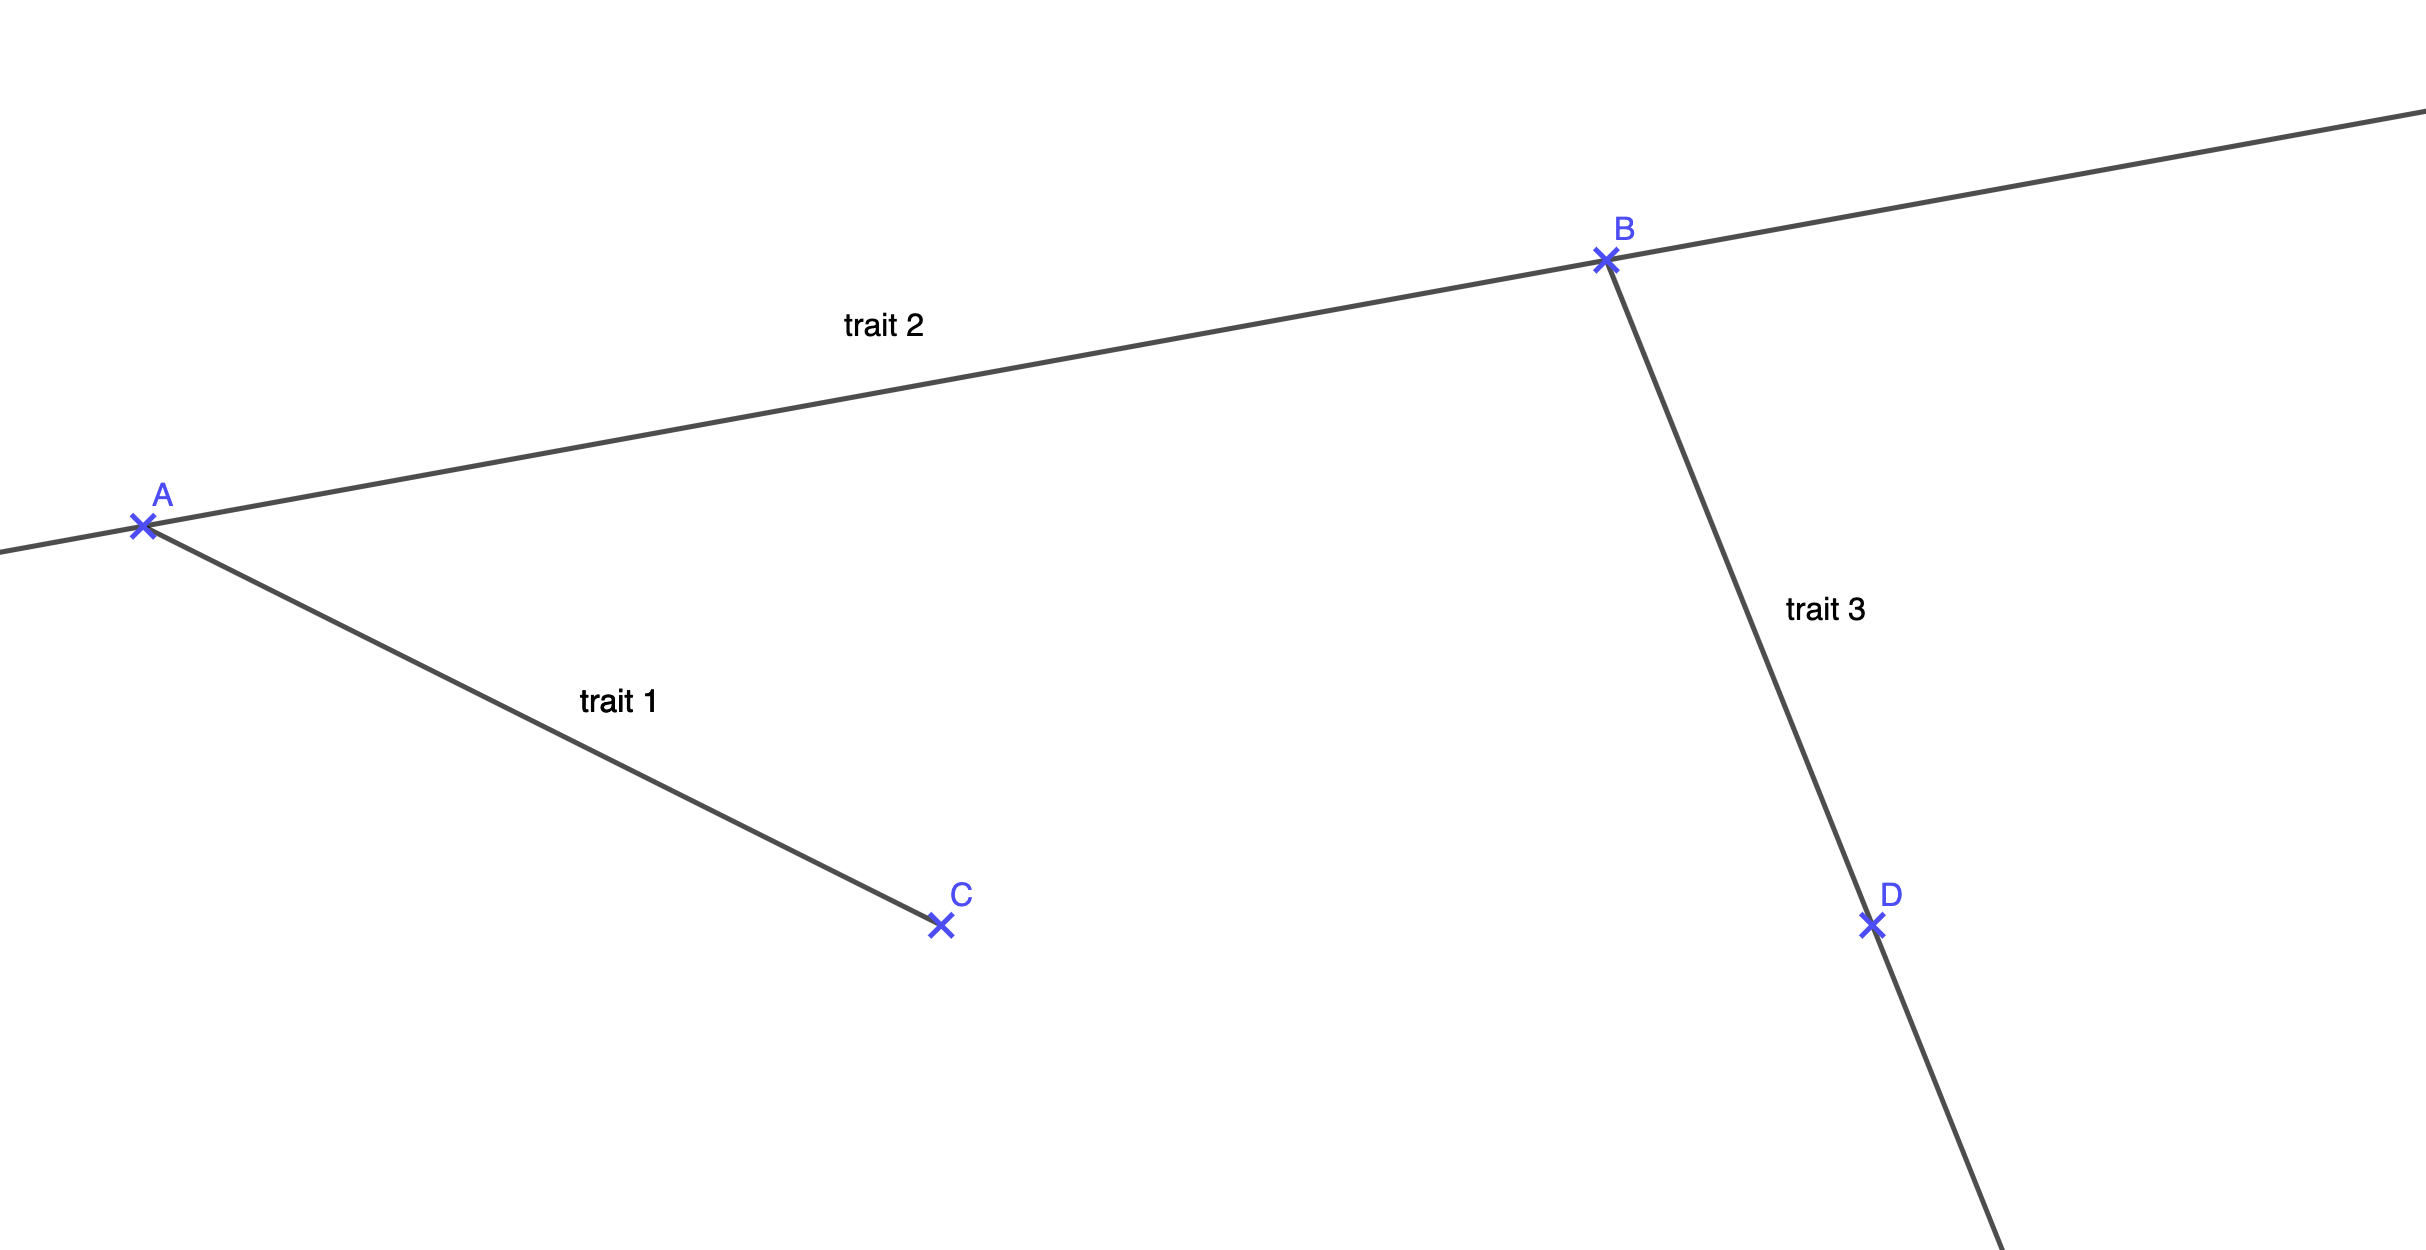
\includegraphics[scale=.45]{Fig1}\]
    
    \subsection*{Exercice 4}
On considère les deux figures suivantes : 

\begin{figure}[H]
\center 
\begin{tikzpicture}[scale =1.3]
\draw (-2, 0) -- (2, 0) arc (0: 180 :2);
\draw (-2, 0) -- (2, 0) arc (0: 180 :2);
\draw[<->] (-2, -.2) -- (2, -.2); 
\draw (0, -.5) node {$7 \ cm$};
\draw[white](0,-1)--(3,-1);
\end{tikzpicture}
\begin{tikzpicture}[scale =1.3]
\draw[dashed](-2, 0) -- (2, 0);
\draw(2,0) arc (0: 180 :2) arc (180:360: 1) arc(180:0:1);
\draw(2,0) arc (0: 180 :2) arc (180:360: 1) arc(180:0:1);
\draw[<->] (2, -.2) -- (0, -.2); 
\draw (1, -.5) node {$4 \ cm$};
\end{tikzpicture}
\end{figure} 
\begin{enumerate}
\item Calculer une valeur exacte du périmètre de la première figure. Donnez ensuite une valeur approchée au millimètre. 

\item Calculer une valeur exacte du périmètre de la seconde figure. Donnez ensuite une valeur approchée au millimètre. 
\end{enumerate} 
 
 
 \newpage
 
\subsection*{Exercice 1 : Calculs}  % 4 points


Posez et effectuez les calculs suivants : 
\begin{enumerate}
\item $23,48 + 95, 91 = $
\item $123,48 - 95, 91 = $
\item $12$ h $51$ min + $4$h $15$ min = 
\item $12$ h $10$ min - $4$h $16$ min =
\item $23,46 + 62, 821 + 134,012 = $
\item $100,01 - 10, 204 =  $
\item $81 \times 12,6 = $
\item $ 23,75 \times 230,75 = $
\end{enumerate}


\subsection*{Exercice 2 : Ordre}

Rangez dans l'ordre croissant les nombres suivants : 
\[ 34,03 ;\ \ \ \  34 + \frac1{10} ;\ \ \ \   \frac{3411}{100} ;\ \ \ \  34,103 ;\ \ \ \   34, + \frac3{100}+\frac1{10}\]

\subsection*{Exercice 3 : Tracé}


Sur la figure suivante, tracez les objets $(AD]$, $[BC]$, et $(CD)$. \\ 
Sur votre copie, nommez les trois traits numérotés de la figure. 
\[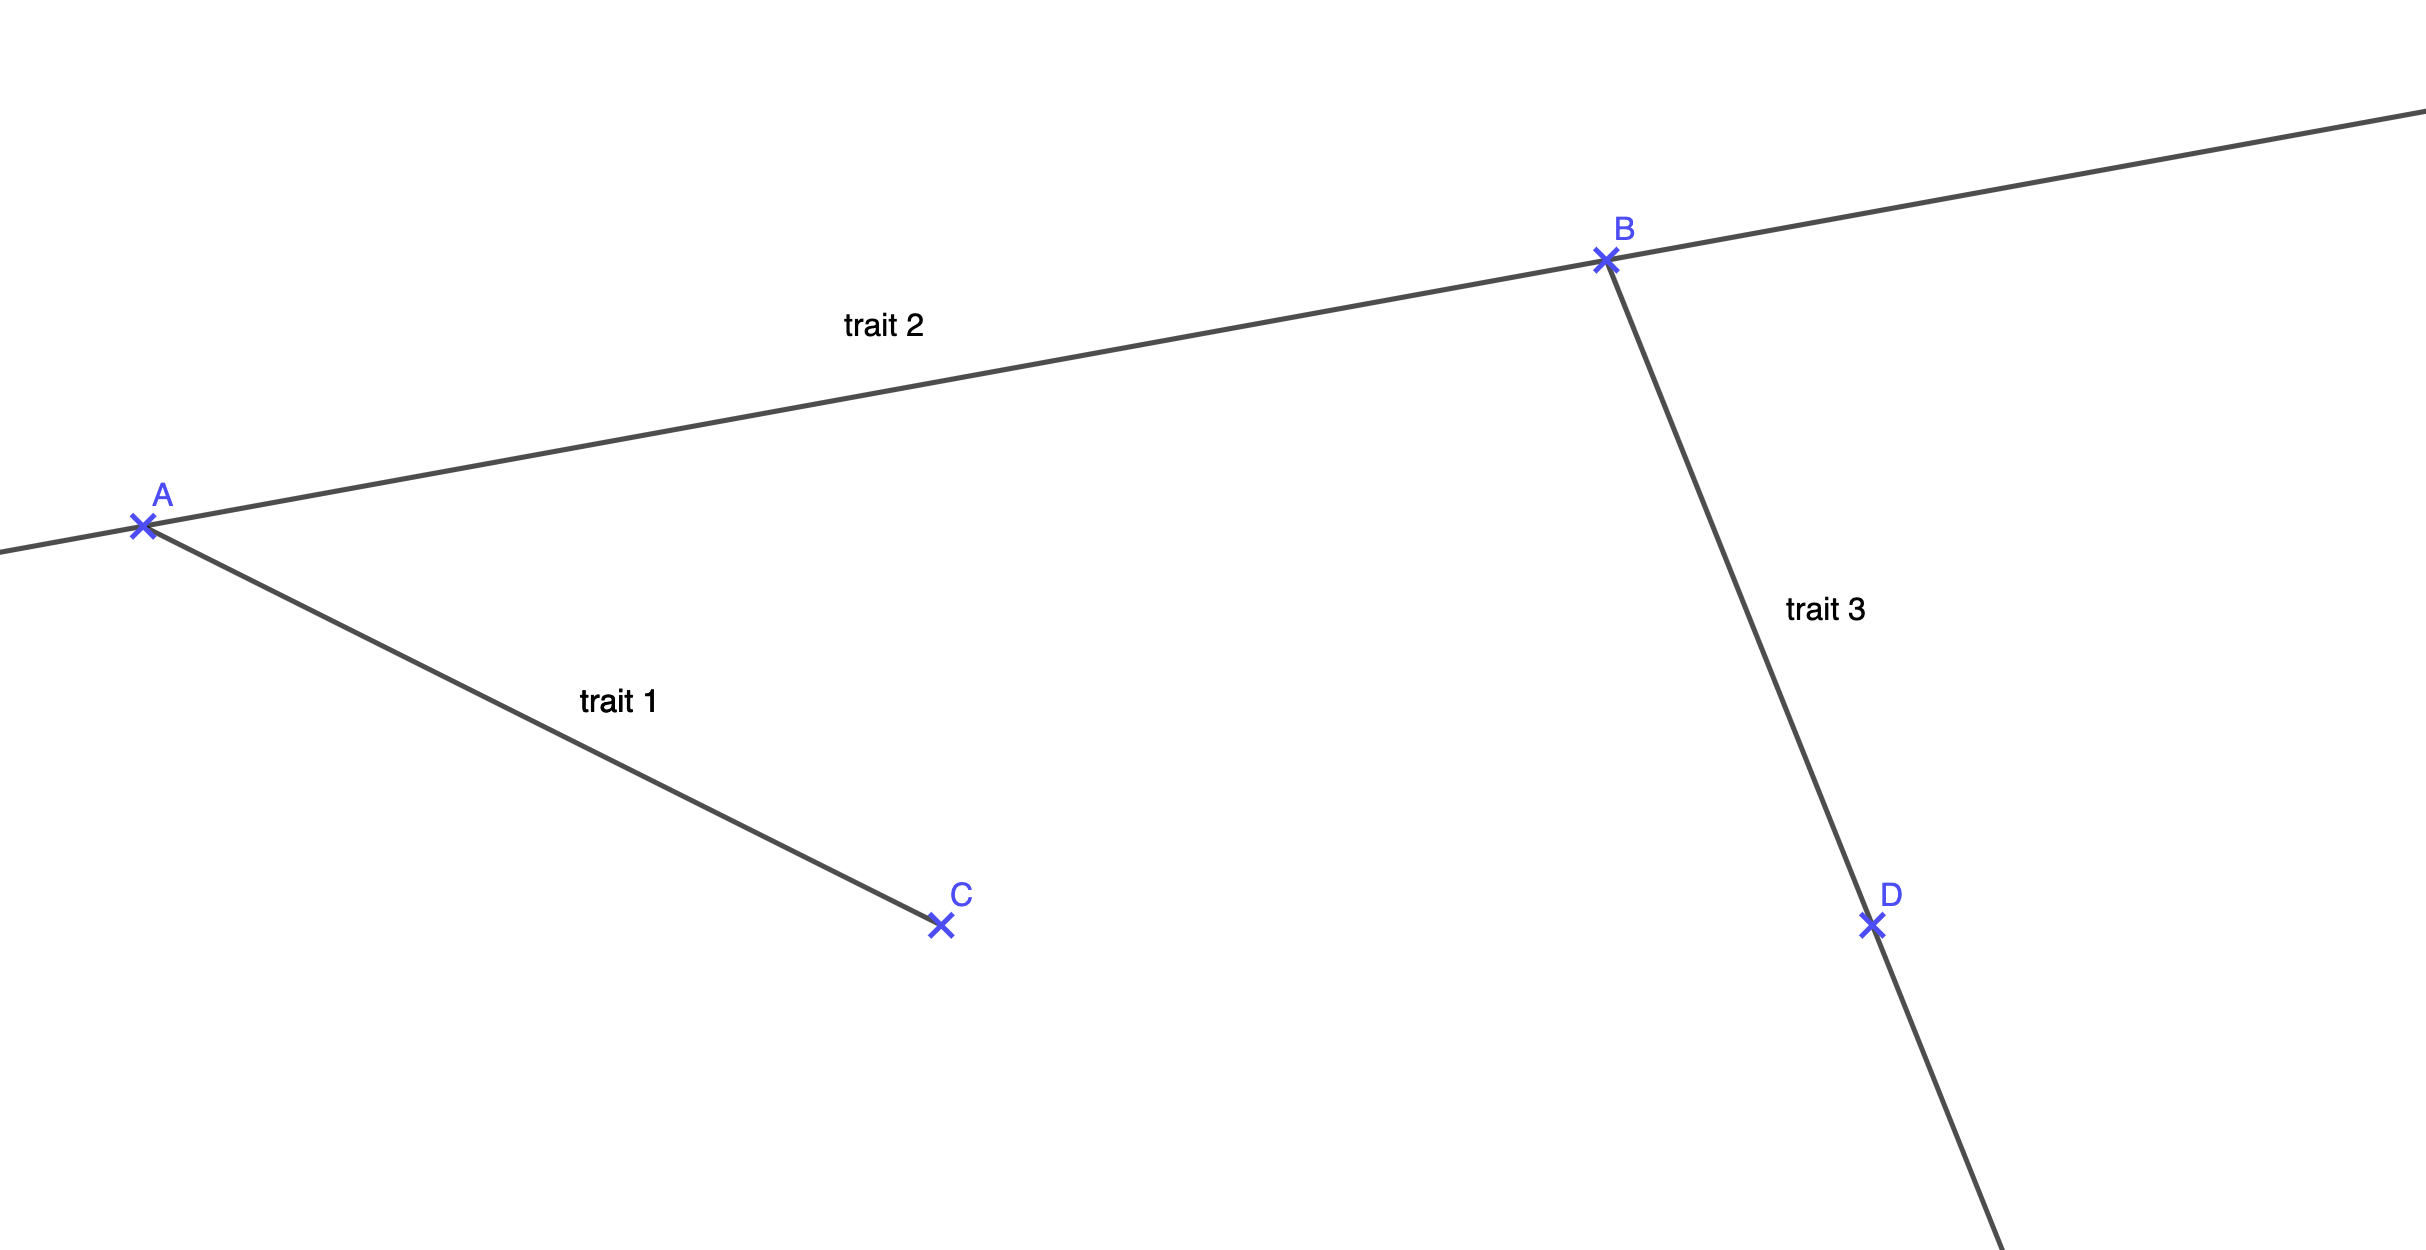
\includegraphics[scale=.45]{Fig1}\]
    
    \subsection*{Exercice 4}
On considère les deux figures suivantes : 

\begin{figure}[H]
\center 
\begin{tikzpicture}[scale =1.3]
\draw (-2, 0) -- (2, 0) arc (0: 180 :2);
\draw (-2, 0) -- (2, 0) arc (0: 180 :2);
\draw[<->] (-2, -.2) -- (2, -.2); 
\draw (0, -.5) node {$6 \ cm$};
\draw[white](0,-1)--(3,-1);
\end{tikzpicture}
\begin{tikzpicture}[scale =1.3]
\draw[dashed](-2, 0) -- (2, 0);
\draw(2,0) arc (0: 180 :2) arc (180:360: 1) arc(180:0:1);
\draw(2,0) arc (0: 180 :2) arc (180:360: 1) arc(180:0:1);
\draw[<->] (2, -.2) -- (0, -.2); 
\draw (1, -.5) node {$4 \ cm$};
\end{tikzpicture}
\end{figure} 
\begin{enumerate}
\item Calculer une valeur exacte du périmètre de la première figure. Donnez ensuite une valeur approchée au millimètre. 

\item Calculer une valeur exacte du périmètre de la seconde figure. Donnez ensuite une valeur approchée au millimètre. 
\end{enumerate} 
 
  
 
 
\end{document}